\section{数值可信性的多重校验}

前四问的结论全部来自同一套离散实现，因此有必要说明这些数字在多大程度上独立于离散参数与实现细节。本章给出四组证据：离散参数的收敛性、与解析解的对照、离散守恒的恒等性，以及一组答案可以先验判定的退化算例。四者的价值在于失效原因互不重叠：收敛性只能说明解对网格与时间步不敏感，却无法排除方程被写错；解析解能查出方程写错，却只在常物性下可用；守恒残差对通量组装的错误极其灵敏，但对系数取值的错误不敏感；退化算例则直接检验极限行为是否正确。

\subsection{离散参数的收敛性与解析解对照}

空间收敛以三个问题各自最敏感的输出量为指标：问题一取表面含水率，因为它位于边界层内、对径向分辨最挑剔；问题三与问题四取停时，因为它是本文的主要交付量。网格由 $N=20$ 加倍到 $40$ 时，三者依次变化 $0.1069\%$、$0.0521\%$、$0.0547\%$，第一项已超出 $0.1\%$ 的容差；再由 $40$ 加倍到 $80$ 时，三者降为 $0.0262\%$、$0.0137\%$、$0.0140\%$，全部远在容差之内。生产网格因此取 $N=40$：更粗一档不能通过检验，更细一档不改变任何一位有效数字。

时间收敛在固定网格上考察。以问题一的中心温度为指标，时间步自 $2$~s 起逐次减半至 $0.25$~s，另在减半序列之外加算一档更细的 $0.1$~s。减半序列内相邻两档之差依次为 $1.202\times10^{-3}$、$6.006\times10^{-4}$、$3.002\times10^{-4}$~°C，每档约为前一档的一半，据此按

\begin{equation}
p=\log_2\frac{y(\Delta t)-y(\Delta t/2)}{y(\Delta t/2)-y(\Delta t/4)},
\qquad
y^{\ast}=y(\Delta t/2)+\frac{y(\Delta t/2)-y(\Delta t)}{2^{p}-1}
\label{eq:order}
\end{equation}

由 $\Delta t=1$、$0.5$、$0.25$~s 这三档算出观测阶为 $1.0005$，与后向 Euler 的理论一阶完全一致；$y$ 对 $\Delta t$ 的线性拟合决定系数为 $0.9999999$，说明高阶残项在该区间内可以忽略。式~\eqref{eq:order} 给出的 Richardson 外推极限为 $33.5752$~°C，与同一支最细的 $\Delta t=0.1$~s 一档相差 $1.2\times10^{-4}$~°C，相对量级为 $10^{-6}$；表~\ref{tab:q1T} 所报的 $33.5753$~°C 与该极限只差末位一个单位。问题三的时间步安排另行考察：恒温平台段由 $120$~s 减半到 $60$~s 使停时变化 $0.0811\%$，生产取值 $60$~s 相对最细的 $10$~s 偏差 $0.0677\%$。网格加倍与时间步减半同时进行时，问题一变化 $0.0291\%$、问题三变化 $0.0544\%$，两项误差没有相互放大。

解析解对照需要一个有闭式答案的算例，因此另设一支：物性取常值、空气温度冻结在实测平台值 $49.9989$~°C，此时热方程退化为常系数线性问题，圆柱在第三类边界下的经典级数解为

\begin{equation}
\frac{T(r,t)-T_a}{T_0-T_a}
=\sum_{n=1}^{\infty}\frac{2\,{\rm Bi}_h}{(\zeta_n^{2}+{\rm Bi}_h^{2})J_0(\zeta_n)}
\,J_0\!\left(\frac{\zeta_n r}{R_0}\right)
\exp\!\left(-\frac{\zeta_n^{2}\alpha t}{R_0^{2}}\right),
\label{eq:bessel}
\end{equation}

式~\eqref{eq:bessel} 中特征值 $\zeta_n$ 取 $\zeta J_1(\zeta)={\rm Bi}_h J_0(\zeta)$ 的正根，前三个为 $1.4185$、$4.1665$、$7.2085$。取十项求和，$1800$~s 时中心温度的解析值为 $43.9623$~°C、表面为 $46.6376$~°C。需要说明的是这一数值与表~\ref{tab:q1T} 的 $33.5753$~°C 并不矛盾：后者的空气温度按附件 1 实测逐时刻变化、半小时内尚在升温途中，而此处为构造闭式解把空气温度整段固定在平台值，两者是不同的算例。数值解在 $N=80$ 上把时间步由 $1$~s 减到 $0.05$~s，中心温度与解析值的绝对偏差由 $3.94\times10^{-3}$~°C 单调降到 $2.20\times10^{-4}$~°C，相邻档之间的观测阶为 $0.99$、$0.97$、$0.92$。三组证据画在图~\ref{fig:verification} 中。

\begin{figure}[htbp]
  \centering
  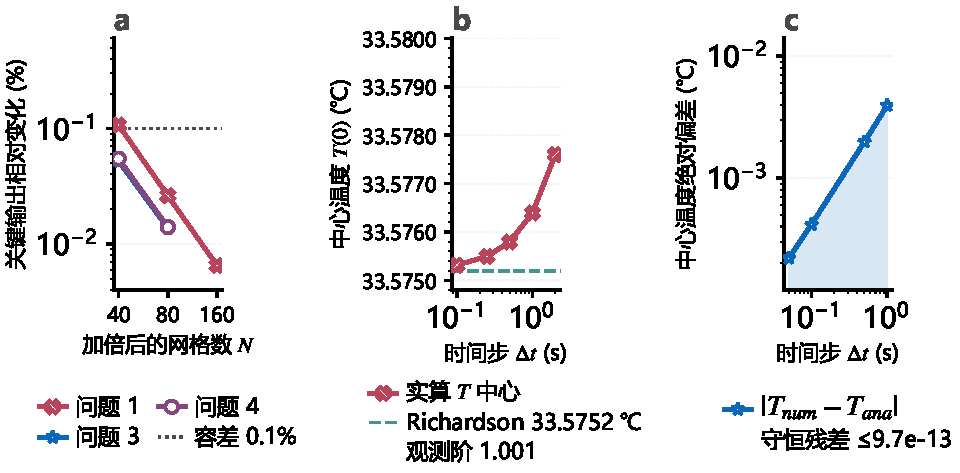
\includegraphics[width=0.9\textwidth,height=0.8\textheight,keepaspectratio]{../figures/fig_verification.pdf}
  \caption{数值可信性三联校验。a：三个问题的关键输出随网格逐次加倍的相对变化，
  仅问题一最粗的一档在 0.1\% 容差线之上，生产网格 $N=40$ 及其后各档均落在线下；
  b：固定网格下中心温度随时间步收敛，观测阶约为 1，
  与后向 Euler 的理论一阶一致，虚线为 Richardson 外推极限；c：常物性算例与十项
  Bessel 级数解析解的中心温度绝对偏差随时间步单调下降。三项合起来说明所报结果
  不依赖离散参数的具体取法。}
  \label{fig:verification}
\end{figure}

左图三条折线都随网格加密单调下行且无回折，在两条停时曲线覆盖的各档上它们都低于含水率那条，这与停时是时间积分量、局部误差在积分中相互抵消的预期一致。中图的数据点排在一条过原点的直线上，斜率即一阶误差常数，外推极限落在直线与纵轴的交点，图上可以直接读出生产取值与该极限的距离。右图的偏差随时间步单调下降且没有出现平台，说明在所考察的区间内误差仍由时间离散主导；固定时间步而把网格由 $40$ 加密到 $160$ 时偏差仅由 $2.93\times10^{-4}$ 降到 $2.02\times10^{-4}$~°C，比值 $1.45$ 远小于时间步方向的下降幅度，这从另一侧印证了同一判断。

\subsection{离散守恒的恒等性及其诊断作用}

守恒检验取单位长度截面的水分总量。以物质测度写出的总量与表面累积失水应当逐时刻相抵，残差定义为

% 两式并排会超出版心 14.8pt，改为上下两行（仍是同一个编号，正文按 eq:massres 引用）。
\begin{equation}
\begin{aligned}
m(t)&=\int_0^1 C(s,t)\,s\,\mathrm{d}s,\\
\varepsilon_{\rm mass}&=\frac{1}{m(0)}\left|\,m(0)-m(t_{\rm end})
-\int_0^{t_{\rm end}}\frac{h_m}{R(t)}\big[C(1,t)-C_a(t)\big]\,\mathrm{d}t\,\right| .
\end{aligned}
\label{eq:massres}
\end{equation}

全部 $33$ 个算例的残差落在 $[0,\ 9.676\times10^{-13}]$ 区间内，容差为 $1\%$，实际值小了十个数量级以上。这一结果并非偶然：控制体体积按式~\eqref{eq:vol} 精确积分而非近似求和，内部界面通量在相邻两个控制体中以相反符号成对出现并逐项相消，因此式~\eqref{eq:massres} 在本离散下是一个代数恒等式，唯一的残差来源是浮点舍入。

正因为它是恒等式，这项检验的用处不在确认物理，而在于定位实现错误：任何破坏成对相消的编码疏漏都会使残差从 $10^{-13}$ 跳到有效数字量级，无法被掩盖。第~\ref{sec:q34} 小节记录的实验室坐标对照支正是这样被查出的，其残差达 $30.3\%$，而单看它给出的停时 $52.6377$~h 与主模型只差 $2.93\%$，凭数值本身根本无法判断对错。

同一处也需要如实记下一项未尽之处。式~\eqref{eq:massres} 中的测度 $s\,\mathrm{d}s$ 与时间无关，因为它计的是干物质份额，而收缩不改变干物质，所以水分方程在收缩域上仍严格守恒。能量方程没有同样的结构：热容项的物理测度含有 $R^2(t)$，本文的离散把该因子并入系数而未追加 $\mathrm{d}(R^2)/\mathrm{d}t$ 一项，因此收缩域上的能量并非严格守恒，本文也不作此宣称。本文未直接估计该项的大小，只能给出一个旁证：把温度场整段冻结为空气温度这一远比之更粗暴的处理，只使停时变化 $0.15\%$，说明在本题的参数下温度场对停时的作用本就很弱，因而这一处理上的疏漏难以经由温度耦合显著改变停时。

\subsection{答案可先验判定的退化算例}

最后一组检验的特点是答案在计算之前就已知道，因此任何偏离都是实现错误而非物理。第一个算例把表面传质系数置零，此时水分无处可去，含水率必须处处保持初值。实算的最大偏离为 $7.1\times10^{-15}$~kg/kg，累积失水恰为零，而温度仍照常升到 $49.97$~°C——两个场没有互相污染，它们之间唯一的联系确实只是扩散系数中的温度因子。

第二个算例把空气条件整段固定在药材的初始状态，即空气温度 $28$~°C、空气水分浓度 $2.55$~kg/kg。此时初始条件本身就是方程的不动点，解不应有任何演化。实算的温度偏离为 $2.5\times10^{-14}$~°C、含水率偏离为 $7.1\times10^{-15}$~kg/kg，守恒残差恰为零，说明两个 Robin 边界的符号与系数都装配正确，没有引入寄生源项。

第三个算例关掉收缩而让两种坐标写法同时运行。$\dot R\equiv0$ 时式~\eqref{eq:chain} 的表观对流项恒为零，两支必须逐位一致。实算给出的截面平均含水率、中心值、表面值与守恒残差在输出的全部位数上完全相同，两支残差均为 $2.6\times10^{-16}$。这一结果把实验室坐标支 $30.3\%$ 残差的来源收窄到收缩项：该支在 $\dot R\equiv0$ 这一极限下未暴露任何差异，故差异只能来自与收缩相关的项，复查确认为收缩效应被计入两次。

% 本段行内数学最密（含 0.5000000000000001 这类不可断长串），额外给出应急伸展量。
{\emergencystretch=3em
第四个算例考察长时间极限。把物性冻结、空气水分浓度固定在平台值 $0.049988$~kg/kg 并推进到 $7.2\times10^5$~s，截面平均含水率应单调降至空气值而不越过。实算终值为 $0.049988$~kg/kg，全程的最大回升量为 $-1.1\times10^{-16}$，即没有出现任何回升，且各时刻的最小含水率始终不低于空气值。第三类边界确实把解驱动到平衡而不是驱动过头。此外，同一线性系统分别用 Thomas 追赶法与带状直接解求出，最大差别为 $2.2\times10^{-16}$；控制体体积之和为 $0.5000000000000001$，与解析值 $1/2$ 相差一个机器精度单位。\par}

四组证据的覆盖面各有边界：解析对照只验证常物性线性情形，退化算例只验证答案先验已知的极限，守恒校核只对破坏成对相消的疏漏灵敏。它们合起来说明的是，在这些可判定的情形下离散与实现没有暴露出偏差，因此本文认为主要的不确定性来自模型选择与参数取值，而非离散精度。这两方面分别用横向对比与扰动分析考察。
